\definecolor{myblue}{RGB}{166, 189, 219}
\definecolor{mygray}{RGB}{211, 211, 211}
\definecolor{mypink}{RGB}{255, 166, 201}

\definecolor{indianred19364103}{RGB}{193,64,103}
% \definecolor{lightgray204}{RGB}{204,204,204}
\definecolor{steelblue51132141}{RGB}{51,132,141}
\definecolor{mygreen}{RGB}{115, 144, 114}
\definecolor{myorange}{RGB}{233, 179, 132}
\definecolor{myred}{RGB}{255, 138, 138}
\definecolor{myviolet}{RGB}{129, 116, 160}

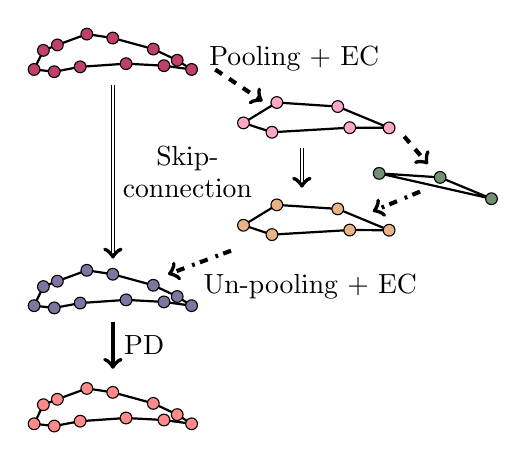
\begin{tikzpicture}[scale=1]

        \def\scaleFactor{2} % Define scaling factor
        \def\circleDia{1.5}
        \def\yShiftInput{0}
        \def\xShift{0}
        
        % Define the points for the input airfoil shape with scaling
        \coordinate (P0) at ({\xShift + \scaleFactor * 0.9996}, {\yShiftInput + \scaleFactor * 0.0008});
        \coordinate (P1) at ({\xShift + \scaleFactor * 0.9083}, {\yShiftInput + \scaleFactor * 0.0590});
        \coordinate (P2) at ({\xShift + \scaleFactor * 0.7565}, {\yShiftInput + \scaleFactor * 0.1303});
        \coordinate (P3) at ({\xShift + \scaleFactor * 0.4992}, {\yShiftInput + \scaleFactor * 0.2004});
        \coordinate (P4) at ({\xShift + \scaleFactor * 0.3345}, {\yShiftInput + \scaleFactor * 0.2253});
        \coordinate (P5) at ({\xShift + \scaleFactor * 0.1474}, {\yShiftInput + \scaleFactor * 0.1564});
        \coordinate (P6) at ({\xShift + \scaleFactor * 0.0586}, {\yShiftInput + \scaleFactor * 0.1220});
        \coordinate (P7) at ({\xShift + \scaleFactor * -0.0004}, {\yShiftInput + \scaleFactor * 0.0008});
        \coordinate (P8) at ({\xShift + \scaleFactor * 0.1276}, {\yShiftInput + \scaleFactor * -0.0135});
        \coordinate (P9) at ({\xShift + \scaleFactor * 0.2922}, {\yShiftInput + \scaleFactor * 0.0174});
        \coordinate (P10) at ({\xShift + \scaleFactor * 0.5837}, {\yShiftInput + \scaleFactor * 0.0376});
        \coordinate (P11) at ({\xShift + \scaleFactor * 0.8242}, {\yShiftInput + \scaleFactor * 0.0246});
        \coordinate (P12) at ({\xShift + \scaleFactor * 0.9996}, {\yShiftInput + \scaleFactor * 0.0008});
        
        % Draw the airfoil shape
        \draw[thick] (P0) -- (P1) -- (P2) -- (P3) -- (P4) -- (P5) -- (P6) -- (P7) -- (P8) -- (P9) -- (P10) -- (P11) -- (P12) -- cycle;
        
        % Add circles at selected points
        \foreach \i in {1, 2, 3, 4, 5, 6, 7, 8, 9, 10, 11, 12} {
            \node[circle, draw, fill=indianred19364103, inner sep=\circleDia pt] at (P\i) {};
        }
    
        % skip at decoded graph
        \draw[->, double, black, line width=0.5pt, double distance=0.5pt](1, -0.2 + \yShiftInput) -- (1,-2.4 + \yShiftInput)
        node[midway, right] {\shortstack{Skip-\\connection}};
        % {\shortstack{Pressure Decoder \\ (PD)}};
    
        % Define the points for the decoded airfoil shape
        \def\xShift{0}
        \def\yShiftDecoded{-3 + \yShiftInput}
    
        % Define the points for the input airfoil shape with scaling
        \coordinate (P0) at ({\xShift + \scaleFactor * 0.9996}, {\yShiftDecoded + \scaleFactor * 0.0008});
        \coordinate (P1) at ({\xShift + \scaleFactor * 0.9083}, {\yShiftDecoded + \scaleFactor * 0.0590});
        \coordinate (P2) at ({\xShift + \scaleFactor * 0.7565}, {\yShiftDecoded + \scaleFactor * 0.1303});
        \coordinate (P3) at ({\xShift + \scaleFactor * 0.4992}, {\yShiftDecoded + \scaleFactor * 0.2004});
        \coordinate (P4) at ({\xShift + \scaleFactor * 0.3345}, {\yShiftDecoded + \scaleFactor * 0.2253});
        \coordinate (P5) at ({\xShift + \scaleFactor * 0.1474}, {\yShiftDecoded + \scaleFactor * 0.1564});
        \coordinate (P6) at ({\xShift + \scaleFactor * 0.0586}, {\yShiftDecoded + \scaleFactor * 0.1220});
        \coordinate (P7) at ({\xShift + \scaleFactor * -0.0004}, {\yShiftDecoded + \scaleFactor * 0.0008});
        \coordinate (P8) at ({\xShift + \scaleFactor * 0.1276}, {\yShiftDecoded + \scaleFactor * -0.0135});
        \coordinate (P9) at ({\xShift + \scaleFactor * 0.2922}, {\yShiftDecoded + \scaleFactor * 0.0174});
        \coordinate (P10) at ({\xShift + \scaleFactor * 0.5837}, {\yShiftDecoded + \scaleFactor * 0.0376});
        \coordinate (P11) at ({\xShift + \scaleFactor * 0.8242}, {\yShiftDecoded + \scaleFactor * 0.0246});
        \coordinate (P12) at ({\xShift + \scaleFactor * 0.9996}, {\yShiftDecoded + \scaleFactor * 0.0008});
        
        % Draw the airfoil shape
        \draw[thick] (P0) -- (P1) -- (P2) -- (P3) -- (P4) -- (P5) -- (P6) -- (P7) -- (P8) -- (P9) -- (P10) -- (P11) -- (P12) -- cycle;
        
        % Add circles at selected points
        \foreach \i in {1, 2, 3, 4, 5, 6, 7, 8, 9, 10, 11, 12} {
            \node[circle, draw, fill=myviolet, inner sep=\circleDia pt] at (P\i) {};
        }
    
        % Pressure decoder
        \draw[->, thick, black, line width=1.5pt](1,-3.2 + \yShiftInput) -- (1,-3.8 + \yShiftInput)
        node[midway, right] {PD};
    
        % Output airfoil
        \def\xShift{0}
        \def\yShiftOutput{-4.5 + \yShiftInput}
    
        \coordinate (P0) at ({\xShift + \scaleFactor * 0.9996}, {\yShiftOutput + \scaleFactor * 0.0008});
        \coordinate (P1) at ({\xShift + \scaleFactor * 0.9083}, {\yShiftOutput + \scaleFactor * 0.0590});
        \coordinate (P2) at ({\xShift + \scaleFactor * 0.7565}, {\yShiftOutput + \scaleFactor * 0.1303});
        \coordinate (P3) at ({\xShift + \scaleFactor * 0.4992}, {\yShiftOutput + \scaleFactor * 0.2004});
        \coordinate (P4) at ({\xShift + \scaleFactor * 0.3345}, {\yShiftOutput + \scaleFactor * 0.2253});
        \coordinate (P5) at ({\xShift + \scaleFactor * 0.1474}, {\yShiftOutput + \scaleFactor * 0.1564});
        \coordinate (P6) at ({\xShift + \scaleFactor * 0.0586}, {\yShiftOutput + \scaleFactor * 0.1220});
        \coordinate (P7) at ({\xShift + \scaleFactor * -0.0004}, {\yShiftOutput + \scaleFactor * 0.0008});
        \coordinate (P8) at ({\xShift + \scaleFactor * 0.1276}, {\yShiftOutput + \scaleFactor * -0.0135});
        \coordinate (P9) at ({\xShift + \scaleFactor * 0.2922}, {\yShiftOutput + \scaleFactor * 0.0174});
        \coordinate (P10) at ({\xShift + \scaleFactor * 0.5837}, {\yShiftOutput + \scaleFactor * 0.0376});
        \coordinate (P11) at ({\xShift + \scaleFactor * 0.8242}, {\yShiftOutput + \scaleFactor * 0.0246});
        \coordinate (P12) at ({\xShift + \scaleFactor * 0.9996}, {\yShiftOutput + \scaleFactor * 0.0008});
        
        % Draw the airfoil shape
        \draw[thick] (P0) -- (P1) -- (P2) -- (P3) -- (P4) -- (P5) -- (P6) -- (P7) -- (P8) -- (P9) -- (P10) -- (P11) -- (P12) -- cycle;
        
        % Add circles at selected points
        \foreach \i in {1, 2, 3, 4, 5, 6, 7, 8, 9, 10, 11, 12} {
            \node[circle, draw, fill=myred, inner sep=\circleDia pt] at (P\i) {};
        }
    

    % Draw thick arrows:
    % from input to pooled graph
    \draw[->, dashed, thick, black, line width=1.5pt](2.3, 0) -- (3.2 - 0.3, -0.5 + 0.1) 
    node[midway, above, yshift=1pt, xshift=20pt] {\shortstack{Pooling $+$ EC}};
    
    % Define the points for the pooled graph
    \def\xShift{3.2 + 0 - 0.3 - 0.3}
    \def\yShift{-0.5 - 0.3}

    \coordinate (PO0) at ({\xShift + \scaleFactor * 0.9539}, {\yShift + \scaleFactor * 0.0299});
    \coordinate (PO1) at ({\xShift + \scaleFactor * 0.6278}, {\yShift + \scaleFactor * 0.1653});
    \coordinate (PO2) at ({\xShift + \scaleFactor * 0.2409}, {\yShift + \scaleFactor * 0.1909});
    \coordinate (PO3) at ({\xShift + \scaleFactor * 0.0291}, {\yShift + \scaleFactor * 0.0614});
    \coordinate (PO4) at ({\xShift + \scaleFactor * 0.2099}, {\yShift + \scaleFactor * 0.0020});
    \coordinate (PO5) at ({\xShift + \scaleFactor * 0.7039}, {\yShift + \scaleFactor * 0.0311});
    \coordinate (PO6) at ({\xShift + \scaleFactor * 0.9539}, {\yShift + \scaleFactor * 0.0299});
    % Draw the airfoil shape
    \draw[thick] (PO0) -- (PO1) -- (PO2) -- (PO3) -- (PO4) -- (PO5) -- (PO6) -- cycle;

    % Add circles at selected points
    \foreach \i in {1, 2, 3, 4, 5, 6} {
        \node[circle, draw, fill=mypink, inner sep=\circleDia pt] at (PO\i) {};
    }

    % Skip at pooled graph
    \draw[->, double, black, line width=0.5pt, double distance=0.5pt](1 + \xShift - 0.2, -0.2 + \yShift) -- (1 + \xShift - 0.2, -0.7 + \yShift);

    % Define the points for the un-pooled graph
    \def\xShift{3.2 + 0 - 0.3 - 0.3}
    \def\yShift{-0.5 - 0.3 - 1.3}

    \coordinate (PO0) at ({\xShift + \scaleFactor * 0.9539}, {\yShift + \scaleFactor * 0.0299});
    \coordinate (PO1) at ({\xShift + \scaleFactor * 0.6278}, {\yShift + \scaleFactor * 0.1653});
    \coordinate (PO2) at ({\xShift + \scaleFactor * 0.2409}, {\yShift + \scaleFactor * 0.1909});
    \coordinate (PO3) at ({\xShift + \scaleFactor * 0.0291}, {\yShift + \scaleFactor * 0.0614});
    \coordinate (PO4) at ({\xShift + \scaleFactor * 0.2099}, {\yShift + \scaleFactor * 0.0020});
    \coordinate (PO5) at ({\xShift + \scaleFactor * 0.7039}, {\yShift + \scaleFactor * 0.0311});
    \coordinate (PO6) at ({\xShift + \scaleFactor * 0.9539}, {\yShift + \scaleFactor * 0.0299});
    % Draw the airfoil shape
    \draw[thick] (PO0) -- (PO1) -- (PO2) -- (PO3) -- (PO4) -- (PO5) -- (PO6) -- cycle;

    % Add circles at selected points
    \foreach \i in {1, 2, 3, 4, 5, 6} {
        \node[circle, draw, fill=myorange, inner sep=\circleDia pt] at (PO\i) {};
    }

    % from un-pooled graph to decoded graph
    \draw[->, dash pattern={on 3pt off 2pt on 1pt off 3pt}, thick, black, line width=1.5pt] (1 + \xShift - 1 - 0.1, \yShift - 0.3 + 0.1) -- (0 + \xShift - 1 + 0.1, \yShift - 0.3 - 0.2)
    node[midway, below, yshift=0pt, xshift=40pt] {\shortstack{Un-pooling $+$ EC}};

    % from pooled graph to full depth graph
    \def\yShift{-0.5 - 0.3}
    \draw[->, dashed, thick, black, line width=1.5pt](\xShift + 2 + 0.2 - 0.1, 0 + \yShift - 0.05) -- (\xShift + 2 + 0.9 - 0.4 - 0.1, -0.5 + \yShift + 0.1);

    % Define the points for full depth graph
    \def\xShift{4.2 - 0.3}
    \def\yShift{-1.7}
    
    \coordinate (PO0) at ({\xShift + \scaleFactor * 0.9539}, {\yShift + \scaleFactor * 0.0299});
    \coordinate (PO1) at ({\xShift + \scaleFactor * 0.6278}, {\yShift + \scaleFactor * 0.1653});
    \coordinate (PO2) at ({\xShift + \scaleFactor * 0.2409}, {\yShift + \scaleFactor * 0.1909});
    \coordinate (PO3) at ({\xShift + \scaleFactor * 0.9539}, {\yShift + \scaleFactor * 0.0299});

    % Draw the airfoil shape
    \draw[thick] (PO0) -- (PO1) -- (PO2) -- (PO3) -- cycle;

    % Add circles at selected points
    \foreach \i in {1, 2, 3} {
        \node[circle, draw, fill=mygreen, inner sep=\circleDia pt] at (PO\i) {};
    }
    
    % from full depth to un-pooled graph
    \draw[->, dash pattern={on 3pt off 2pt on 1pt off 3pt}, thick, black, line width=1.5pt] (\xShift + 1, \yShift + 0.2 - 0.1 + 0.05) --  (\xShift + 0.4, \yShift - 1 + 0.6 + 0.2 + 0.1);

    \end{tikzpicture}